\documentclass{beamer}
\usefonttheme[onlymath]{serif}
\usepackage{amsmath}
\usepackage{amsfonts}
\usepackage[utf8]{inputenc}

% definitions
\def\X{\mathbf{X}}
\def\w{\mathbf{w}}
\def\W{\mathbf{W}}
\def\const{\mathrm{const}}
\def\Var{\mathrm{Var}}
\def\tr{\mathrm{tr}}
\def\T{\top}
\def\U{\mathbf{U}}
\def\S{\mathbf{S}}
\def\V{\mathbf{V}}
\newcommand{\argmin}{\mathop{\mathrm{argmin}}}
\newcommand{\argmax}{\mathop{\mathrm{argmax}}}
\newcommand{\minimize}{\mathop{\mathrm{minimize}}}
\newcommand{\maximize}{\mathop{\mathrm{maximize}}}
\newcommand{\st}{\mathop{\mathrm{subject\,\,to}}}

%Information to be included in the title page:
\usecolortheme{seahorse}
\title{Component Analysis}
\author{Thomas Bayes}
\institute{
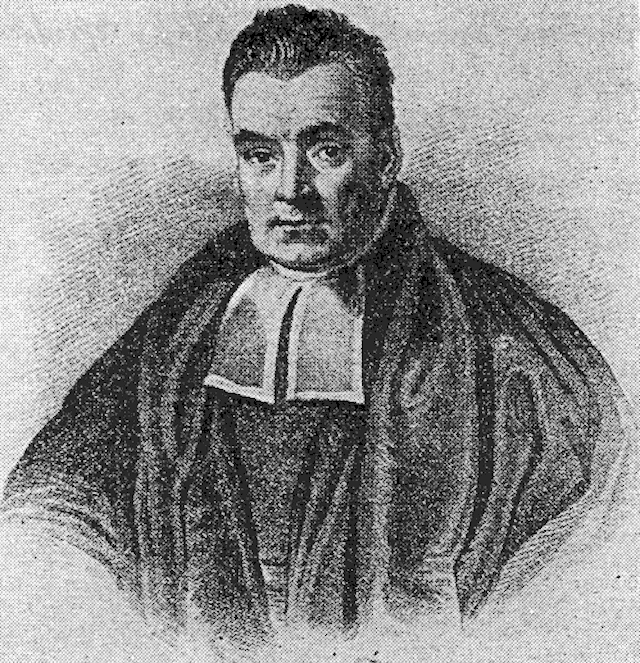
\includegraphics[height=.3\textheight]{../bayes.png}%
}
\date{\today}

    
    
\begin{document}
    
\frame{\titlepage}

\begin{frame}[allowframebreaks]{Principle Component Analysis}
% \frametitle{Principle Component Analysis}
% For $k=1$ dimension case, find direction which maximize variation
% \begin{align*}
% \maximize \Var (\X \w) \\
% = \frac{\w^\T \X^\T \X \w}{n} = \w^\T \Sigma \w
% \end{align*}
Find one direction which minimize reconstruction error,
$$\minimize ||\X - \X \W \W^\T||^2 $$
\begin{align*}
& ||\X - \X \W \W^\T||^2 \\
= \quad & \tr ((\X - \X \W \W^\T) (\X - \X \W \W^\T)^\T) \\
= \quad & \tr(\X \X^\T) - 2 \tr(\X \W \W^\T \X^\T) + \tr (\X \W \W^\T \W \W^\T \X^\T) \\ 
= \quad & \const - \tr (\X \W \W^\T \X^\T) \\
= \quad & \const - \tr (\W^\T \X^\T \X  \W) \\
= \quad & \const - \const \cdot \tr (\W^\T \mathbf{\Sigma} \W)
\end{align*}
This is equivalent to maximizing the total variance of $\X$ on the projected space $\X\W$. \\
\framebreak
Now we show that the solution is the first $k$ eigenvectors of $\mathbf{\Sigma}$. Assume $\X_{n \times d}$ is full rank $d$, SVD decomposition of 
$\X_{n \times d} = \U_{n \times n} \S_{n \times d} \V_{d \times d}^\T$. $$\mathbf{\Sigma} = \X^\T \X = \const \cdot (\V \S^\T \U^\T \U \S \V^\T) = \const \cdot (\V \S^\T \S \V^\T)$$
We denote $\S^\T \S$ as $\mathbf{\Lambda}$, $\tr (\W^\T \mathbf{\Sigma} \W) = \tr (\W^\T \V \mathbf{\Lambda} \V^\T \W)$. Note that $\mathbf{R} = \V^\T \W$ is also a orthonormal matrix. So $$\tr (\W^\T \V \mathbf{\Lambda} \V^\T \W) = \tr (\mathbf{R}^\T \mathbf{\Lambda} \mathbf{R}) = \sum_{i=1}^d \lambda_i \sum_{j=1}^k\mathbf{R}_{ij}^2 \le \sum_{i=1}^k \lambda_i$$

We just pick the largest $k$ eigen values and get the result. \\
\framebreak
So from minimizing reconstruction error using a linear combination subspace, we have showed that it is equivalent to maximizing the total variance of the projection on linear subspace and the correponding subspace is formed of exactly the $k$ largest eigenvectors.(Note that we do not use any other assumpition except linearity.)
\end{frame}



\begin{frame}[allowframebreaks]{Linear Discriminant Analysis}

\end{frame}

\begin{frame}[allowframebreaks]{Independent Component Analysis}
In PCA we mentioned earlier, we want to find a linear combination subspace for which the reconstruction error is minimized. In ICA, we want to find the 
\end{frame}
\end{document}